\lab{Algorithms}{Speeding up MATLAB Functions: Vectorization}{Vectorization}

\objective{Demonstrates the importance of vectorization in MATLAB.}

As we explained in lab 6, MATLAB is highly optimized to do operations on vectors. For this reason, MATLAB is much slower when we use loops and conditionals. This lab introduces two applied topics (Information Entropy and Chebyshev Polynomials) to explore how we can make functions faster through vectorization.

\section*{Information Entropy}

Information entropy is loosely defined as the amount of information that is encoded in each bit of a signal. It is directly related to amount of compression that a signal can undergo without loss.

For example, suppose that our signal is an infinite string ``AAAAAAA...'' Since the signal never changes each bit offers no new information. Thus the entropy in this case is zero.

On the other hand, we assign a truly random uniform binary source an entropy of one (such a source may be related to radioactive decay). This is since we have absolutely no clue what the next symbol we read will be.

We can empirically calculate the entropy of a given signal by the following:
\[
H = -\sum_k{p_k log_2(p_k)}
\]
where $p_k$ is the probability of the kth symbol. Note that this fits the two conventions we set above since
\[
-(1log_2(1) + 0 log_2(0)) = 0
\]
\[
-(1/2log_2(1/2) + 1/2log_2(1/2)) = 1
\]

\begin{problem}
Write a function that finds the entropy of a given input vector {\tt v}. You will have to empirically calculate the probability of a given symbol (you should probably let your symbols be integers). This can be done simply using a {\tt for} loop and the {\tt unique} command.
\end{problem}

We can test the entropy function that you just wrote against bit sources to see how ``random'' they are. For example, we can read an image into MATLAB and view it using the following code:
\begin{verbatim}
>> [X map] = imread('cameraman.tif');
>> imshow(X)
\end{verbatim}

\begin{figure}[h!]
\begin{center}
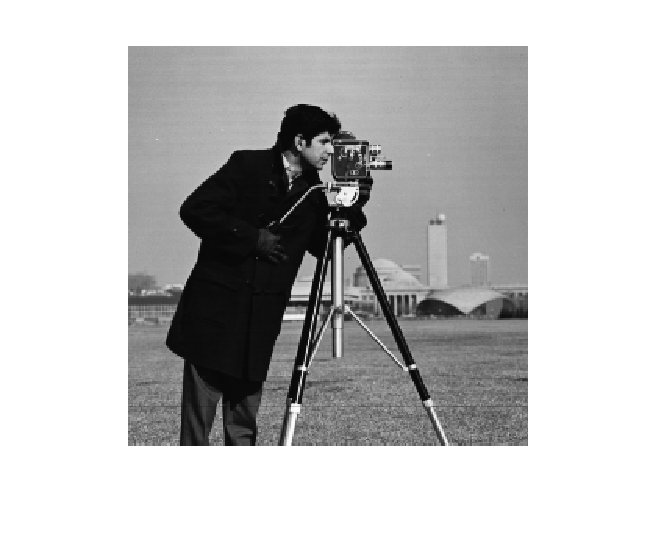
\includegraphics{./Figures/cameramanClean.pdf}
\end{center}
\caption{The MIT camerman, a classic image used in image processing}
\end{figure}
You should see the image shown in figure 1.3. Now run your function on this image (we had to use the code {\tt entropy(X(:)')} to write the signal as a vector). We get a value of $7.009$. If this image were uniformily random, the entropy would be $8$, since each pixel is an $8$ bit number, and a uniform distribution of integers between $1$ and $128 = 2^8$ will have an entropy of $8$ (you can verify this fairly easily using the equation we defined above). This implies that the image has potential for compression.

\begin{problem}
Now rewrite your function without using loops. This is an example of using vectorization to speed up algorithms. Use the cameraman image to test how much faster this function is than your original.
\end{problem}

\section*{Chebyshev Polynomials}

One special type of polynomials are the Chebyshev Polynomials. They are useful in a variety of applications including:
\begin{itemize}
\item Evaluating integrals using Gaussian quadrature
\item Solving PDE's
\item Speeding up iterative matrix methods (finding eigenvalues and solving large systems)
\item minimizing interpolation error
\end{itemize}

We will explain many of the these applications in subsequent chapters. The purpose of this example is primarily to give you a real opportunity to investigate ways to speed a process up on your own.

The value of the n-th chebyshev polynomials can be described by the following mathematical formulae\footnotemark :
\[
T_n(x) = cos(n cos^{-1}(x))
\]

\[
T_n(x) = 2xT_{n-1}(x) - T_{n-2}(x), T_0(x) = 1, T_1(x) = x
\]

\footnotetext{Technically the first formula only works on the interval $[-1,1]$. There are more general formulae, piecewise defined using $cosh$ outside of $[-1,1]$, but for this exercise we'll stick to the above definition.}

\begin{problem}
Write a function that accepts a vector $x_0$ of values in $[-1,1]$ and a degree $n$, and returns a matrix evaluting each entry of $x_0$ at every chebeshev polynomial of degree $n$ or less. Essentially, the n-th column of the output should contain the $n-1$ Chebyshev Polynomial evaluated at $x_0$. Make this function as fast as possible (this is the point of the exercise, writing a function solving this problem shouldn't be too difficult anymore). You should investigate both mathematical definitions, and how the number of {\tt for} loops effects the speed. Explain how you optimized your function, and why other implementations would be slower.
\end{problem}
